The goal of the depth-color fusion algorithm is to find the correspondences between the pixels of a depth 
image and the pixels of a color image that have been acquired with a depth-color camera setup like the one 
described in Section \ref{cameras}. The first step of the algorithm is to retrieve the intrinsic and extrinsic 
parameters from both cameras. This is achieved by performing synchronized camera calibration. 

Given the cameras' parameters, the next step computes the relative transformation between the depth 
and color cameras, which is described in terms of a rotation and a translational offset. The relative 
transformation is used to transform world points in the depth camera's coordinate system to world points in
the color camera's coordinate system. The correspondences between points in the depth image and points 
in the color image are retrieved from an image point to world point transformation, followed by a world point 
to image point transformation.


\subsection{Cameras Calibration} \label{camerascalibration}


The depth and color cameras need to be calibrated in order to retrieve their intrinsic and extrinsic 
parameters. Since the goal is to find how the cameras are positioned and oriented one with respect to the 
other, the calibration of the cameras needs to be performed synchronously. In other words, there needs
to exist a positional correspondence between the calibration images taken with both cameras. This is 
achieved by setting the calibration pattern in a fixed position with respect to the camera setup and capturing 
one image from each camera at the same time. The two synchronized images are called an 
\textit{image pair} (see Figure \ref{imagepair}). 

\begin{figure}[t]
	\center
	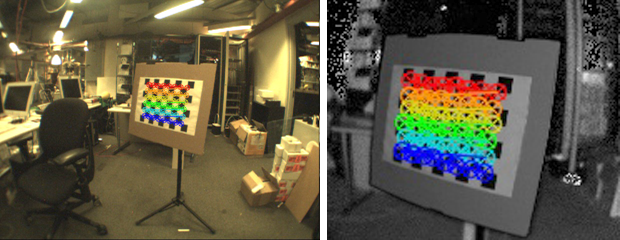
\includegraphics[width = 15cm]{imagepair.png}
	\caption[Example of a calibration image pair]{Example of a calibration image pair. An image pair is 
	composed of a color image (left) and an amplitude image from the depth camera (right).}
	\label{imagepair}
\end{figure}

As observed in Figure \ref{imagepair}, the image pair consists of a color image and an amplitude image. 
Since the amplitude image is visually similar to a grayscale image, it is possible to use it in the calibration 
process to find the calibration pattern. The colored circles in the figure indicate the location of the corners
in the pattern (see Section \ref{calibrationtool}). Besides knowing the correspondence between the images 
in an image pair, the synchronized calibration algorithm needs to know the correspondence between the 
calibration points in the two images.

The calibration process described in Section \ref{calibrationtool} computes the camera's focal length and 
principal point. If $f$ is the focal length of a camera, and $m_x$, $m_y$ are the ratios of pixel width and pixel 
height per unit distance, respectively, then $(f_x, f_y)$ represents the focal length expressed in units of 
horizontal and vertical pixels. That is, 
\begin{align}
(f_x, f_y) = ( f m_x , f m_y)
\end{align}

Furthermore, $(x_0, y_0)$ represents the principal point of the camera. Assuming that the skew coefficient 
between the $x$ and $y$ axes is zero, the intrinsic matrix of this camera is given by 
\begin{align} \label{intrinsicmatrix}
\mathbf{K} = \begin{bmatrix}
	f_x & 0    & x_0 \\
	0    & f_y & y_0 \\
	0    & 0    & 1      \\
\end{bmatrix}
\end{align}

The calibration process also provides a rotation matrix and a translation vector. These parameters describe
the transformation between the world's coordinate system and the camera's coordinate system. If 
$\mathbf{R}$ denotes the $3 \times 3$ rotation matrix, and $\mathbf{t}$ denotes the $3 \times 1$ 
translation vector, the extrinsic matrix of this camera is given by the $3 \times 4$ matrix 
\begin{align} \label{extrinsicmatrix}
\begin{bmatrix} \mathbf{R} & \mathbf{t} \\ \end{bmatrix}
\end{align}

Therefore, the synchronized calibration algorithm outputs two intrinsic matrices, $\mathbf{K}_d$ and 
$\mathbf{K}_c$, and two extrinsic matrices, $[ \mathbf{R}_d ~ \mathbf{t}_d ]$ and 
$[ \mathbf{R}_c ~ \mathbf{t}_c ]$, where the $d$ and $c$ subscripts are used to differentiate between the 
depth camera's parameters and the color camera's parameters. While the intrinsic matrices contain 
information about the internals of the camera, the extrinsic matrices hold information about how the 
cameras are positioned in space. This information is used in the next section to compute the relative 
transformation between both cameras. 


\subsection{Relative Transformation} \label{relativetransformation}


When computing the relative transformation between the cameras, the direction of the transformation is 
chosen to be from the depth camera to the color camera. As discussed in Section \ref{cameras}, the field
of view of the depth camera is within the field of view of the color camera. Therefore, every point in the depth
image will have a corresponding point in the color image, but not necessarily vice versa.

If $\mathbf{P} = (X, Y, Z)^T$ is a point in world coordinates, the position of $\mathbf{P}$ in the depth 
camera's coordinate system is given by $\mathbf{q}_d$. Similarly, the position of $\mathbf{P}$ in the color 
camera's coordinate system is given by $\mathbf{q}_c$. The points $\mathbf{q}_d$ and $\mathbf{q}_c$ 
can be expressed in terms of the cameras' extrinsic parameters by equations \eqref{qd} and \eqref{qc}, 
respectively.
\begin{align}
\mathbf{q}_d = \mathbf{R}_d \mathbf{P} + \mathbf{t}_d	\label{qd} \\
\mathbf{q}_c = \mathbf{R}_c \mathbf{P} + \mathbf{t}_c  	\label{qc}
\end{align}

Considering now the image of $\mathbf{P}$ in the depth image as having coordinates $(x_d, y_d)$, this
point can be expressed in homogeneous coordinates as $\mathbf{p}_d = (w x_d, w y_d, w )^T$, for some 
constant $w$. Using the depth camera's intrinsic parameters, $\mathbf{p}_d$ can be expressed by the 
equation:
\begin{align}
	\mathbf{p}_d = \mathbf{K}_d \mathbf{q}_d \label{pd}
\end{align}

This automatically reveals another expression for $\mathbf{q}_d$:
\begin{align}
	\mathbf{q}_d  = \mathbf{K}_{d}^{-1} \mathbf{p}_d \label{qd2}
\end{align}

Combining the two expressions for $\mathbf{q}_d$ (equations \eqref{qd} and \eqref{qd2}), and solving for 
$\mathbf{P}$ gives an equation for point $\mathbf{P}$:
\begin{align}
	\mathbf{K}_{d}^{-1} \mathbf{p}_d &= \mathbf{R}_d \mathbf{P} + \mathbf{t}_d \nonumber \\
	\mathbf{R}_d \mathbf{P} &= \mathbf{K}_{d}^{-1} \mathbf{p}_d - \mathbf{t}_d  \nonumber \\
	\mathbf{P} &= \mathbf{R}_{d}^{-1} \mathbf{K}_{d}^{-1} \mathbf{p}_d - \mathbf{R}_{d}^{-1} \mathbf{t}_d  
\end{align}

This expression for $\mathbf{P}$ can be substituted in equation \eqref{qc} to get a new expression for 
$\mathbf{q}_c$:
\begin{align}
	\mathbf{q}_c &= \mathbf{R}_c (\mathbf{R}_{d}^{-1} \mathbf{K}_{d}^{-1} \mathbf{p}_d 
					- \mathbf{R}_{d}^{-1} \mathbf{t}_d  ) + \mathbf{t}_c \nonumber \\
			    & =  \mathbf{R}_c \mathbf{R}_{d}^{-1} \mathbf{K}_{d}^{-1} \mathbf{p}_d
			    		 - \mathbf{R}_c \mathbf{R}_{d}^{-1} \mathbf{t}_d + \mathbf{t}_c \label{qc2}
\end{align}

Using equation \eqref{qd2}, equation \eqref{qc2} simplifies to:
\begin{align}
	\mathbf{q}_c &=  (\mathbf{R}_c \mathbf{R}_{d}^{-1}) ~ \mathbf{q}_{d}  
		+ (\mathbf{t}_c - \mathbf{R}_c \mathbf{R}_{d}^{-1} \mathbf{t}_d) \label{qc3}
\end{align}

Equation \eqref{qc3} reveals how the world points in the depth camera's coordinate system are related to 
the world points in the color camera's coordinate system. As seen from the equation, this
transformation is given in terms of the cameras' extrinsic parameters. Therefore, the relative transformation
between the depth and color cameras is defined by the rotation matrix in equation \eqref{relativerotation}
and the translation vector in equation \eqref{relativetranslation}.
\begin{align}
	\mathbf{R}_r = \mathbf{R}_c \mathbf{R}_{d}^{-1} \label{relativerotation} \\
	\mathbf{t}_r = \mathbf{t}_c - \mathbf{R}_r \mathbf{t}_d \label{relativetranslation}
\end{align}


\subsection{Point Correspondences} \label{pointcorrespondences}


The fusion algorithm must convert every point $(x_d, y_d)$ in the depth image into a point $(x_c, y_c)$ in 
the color image. This is achieved by first computing the world point $\mathbf{q}_d$ from the depth image
point $(x_d, y_d)$. Then, $\mathbf{q}_d$ is transformed into $\mathbf{q}_c$ using the results from Section 
\ref{relativetransformation}. Finally, world point $\mathbf{q}_c$ is converted into a color image point 
$(x_c, y_c)$.

If $(f_x, f_y)$ and $(x_0, y_0)$ are the focal length and principal point of the depth camera, respectively, 
the world point $\mathbf{q}_d = (X, Y, Z)^T$ can be related to the image point $(x_d, y_d)$ through the 
perspective projection equations \eqref{xd} and \eqref{yd}. 
\begin{align}
	x_d &= f_x \frac{X}{Z} + x_0 \label{xd} \\
	y_d &= f_y \frac{Y}{Z} + y_0 \label{yd} 
\end{align}
	
The depth camera provides the $z$-component of $\mathbf{q}_d$.\footnote{The depth camera can actually 
provide all components as discussed in Section \ref{cameras}. However, the noise in these measurements is 
high and recomputing the $x$ and $y$ components delivers better results.}
The $x$ and $y$ components are computed by solving equations \eqref{xd} and \eqref{yd} for $X$ and 
$Y$, respectively:
\begin{align}
	X = \frac{Z}{f_x} (x_d - x_0) \label{X} \\
	Y = \frac{Z}{f_y} (y_d - y_0) \label{Y}
\end{align}

Using the color camera's intrinsic parameters, $\mathbf{p}_c$ can be expressed by the equation
\begin{align}
	\mathbf{p}_c = \mathbf{K}_c \mathbf{q}_c \label{pc}
\end{align}

Furthermore, equation \eqref{qc3} gives an expression for $\mathbf{q}_c$. Therefore, combining 
\eqref{pc} and \eqref{qc3} results in a new equation for $\mathbf{p}_c$:
\begin{align}
	\mathbf{p}_c &=  \mathbf{K}_c (\mathbf{R}_r \mathbf{q}_{d}  + \mathbf{t}_r) \label{pc2}
\end{align}

By expressing $\mathbf{q}_{d}$ in homogeneous coordinates (that is, $\mathbf{q}_{d}^{'} = (X, Y, Z, 1)^T$), 
equation \eqref{pc2} can be rewritten as 
\begin{align}
	\mathbf{p}_c &=  \mathbf{K}_c [\mathbf{R}_r  ~  \mathbf{t}_r] \mathbf{q}_{d}^{'} \label{pc3}
\end{align}

The image coordinates $(x_c, y_c)$ are obtained by dividing the first and second components of 
$\mathbf{p}_c$ by its third component. That is, if $\mathbf{p}_c = (x,y,z)^T$, then 
\begin{align}
	(x_c, y_c) = \Bigg( \frac{x}{z} , \frac{y}{z} \Bigg) \label{xcyc}
\end{align}


